\chapter{\label{sec:general_intro}Properties of DNA}

Every known biological cell uses \emph{deoxyribonucleic acid}, in short DNA, 
\nomenclature{DNA}{Deoxyribonucleic acid\refpage}%
as carrier of its hereditary information. DNA is a double stranded heteropolymer into which 
information can be coded by the sequence of its four elementary subunits
known as bases or nucleotides. The information encoded in DNA has
three primary functions. First of all, DNA codes for proteins. The structure of a
protein is determined by its amino acid sequence, which
 is coded as a nucleotide sequence in DNA.
Most organisms known use 20 different amino acids to build their proteins. 
Since there are only four different bases, a multi-letter code has to be used to describe
a sequence of amino acids by a DNA sequence. Biology uses three successive bases,
called \emph{codons},
\nomenclature{Codon}{The genetic code associates with three consecutive bases in DNA one specific amino acid. One element of the genetic code is known as codon}%
to code for one amino acid. To produce a protein, 
the double stranded DNA is locally opened and the nucleotide sequence is transcribed by a protein 
complex called \emph{polymerase} %
\nomenclature{Polymerase}{Protein complex that transcribes DNA into a complementary RNA or DNA strand}
into messenger RNA (mRNA). The mRNA is then translated into a sequence of amino acids, which folds into the functional protein.  
\nomenclature{RNA}{Ribonucleic acid. The structure of RNA and DNA are very similar. 
RNA nucleotides are made from a the sugar ribose instead of desoxyribose.
The base complementary to adenine is uracil instead of thymine} %
\nomenclature{mRNA}{Messenger RNA. Messenger RNAs are transcripts of genes 
that are translated into protein by the ribosome}%
In addition to being the storage medium for protein sequences, DNA has a pivotal role in 
cellular information processing. At every instant in time, a cell has to determine how much of each gene 
is to be expressed. To accomplish this feat, DNA contains 
regulatory regions to which specialized proteins, so called transcription 
factors (TF), can bind. These proteins either preclude or
\nomenclature{TF}{Transcription factor. Transcription factors are specialized proteins that bind to 
DNA and to regulate gene expression}%
enhance the assembly of the transcription machinery and thereby regulate the expression of genes. 
Different signals associated with different TFs can be logically combined by arranging their binding
sites on the DNA such that the TFs bind cooperatively or exclude each other \cite{Gerland_PNAS_02, Buchler_PNAS_03}.
Yet a different class of DNA regions codes for RNA sequences that are not translated into
proteins but have important functions themselves. RNA can form complicated 
secondary and tertiary structures, which make certain RNA molecules powerful catalysts.  
For example the ribosome, the cellular machine that translates the RNA into proteins, 
is a complex of folded RNA molecules and proteins. Its catalytic activity is performed by RNA parts and the 
proteins merely stabilize the RNA complex. Another important example are transfer RNAs (tRNA)
that decipher the genetic code into amino acids. 
\nomenclature{Ribosome}{The ribosome is a RNA-protein complex that translates the mRNA into proteins}%
In addition to these three roles, many other and to date unknown functions of DNA might exist.
Indeed, only a fraction of the genome of higher organism can be linked to any function,
whereas the role of the largest part, often referred to as junk DNA, is largely unknown \cite{HumanGenome_Nature_01}. 
For a comprehensive and fairly up-to-date source of information on molecular biology, I refer the reader to 
the classic textbook by \citeauthor{Alberts_02}

The objectives of this thesis are dynamical aspects of DNA. On one hand, we are going
to discuss the dynamics of the base pairing pattern of two complementary 
DNA strands, whose sequence is the multi-fold repetition of units of one to six
bases in length. Such repetitive sequences play important roles in various processes in biology and 
are related to a certain class of human hereditary diseases. 
What distinguishes them from sequences without this specific order is the dynamics of the 
base pairing pattern which renders repetitive sequences hyper-variable in evolution.
On the other hand, we will study the dynamics of DNA on a much larger scale. 
In eukaryotes DNA is highly compactified. However, in order
to be of any use for the cell, the information encoded in the DNA sequence needs
to be accessible for read out. In chapter \ref{sec:nucleosome}, we will discuss physical aspects of the dynamics of 
compactified DNA, which has profound implication to the accessibility of genetic 
information in eukaryotes.

Since the dominant theme of this thesis is DNA and since its chemical and
physical properties are needed throughout, we will
compile the basics of DNA in this introductory chapter. 
%To begin with, we briefly
%describe its chemical composition and the interaction between its constituents. This
%will be followed by a discussion of the thermodynamic and mechanical properties of DNA. 
%This introductory section 
We will only discuss aspects that are related or prerequisite 
to our work and we do not attempt to provide a comprehensive survey. 
The biological background and the relevance of the specific questions we address is discussed in the 
introductory part of the two main chapters of the thesis. 

\section{\label{sec:DNA_structure}The structure of DNA}
The elementary subunits of DNA are  single nucleotides, which can be 
connected to each other to form a polymer. Each nucleotide consists of 
the sugar \emph{deoxyribose}, a \emph{phosphate group} and one of the four bases 
\emph{adenine} (\basepair{A}), \emph{cytosine} (\basepair{C}), \emph{guanine} (\basepair{G}) and \emph{thymine} (\basepair{T}),
cf.~\FIG{nucleotides}. The phosphate group is attached to the 5' carbon atom
of the sugar. 
\nomenclature{Nucleotide}{Nucleotides are the elementary building blocks of RNA or DNA. 
They consist of a sugar, one or several phosphates and a base\refpage}%
\nomenclature{\basepair{A}}{Adenine\refpage}%
\nomenclature{\basepair{T}}{Thymine\refpage}%
\nomenclature{\basepair{C}}{Cytosine\refpage}%
\nomenclature{\basepair{G}}{Guanine\refpage}%
%Nucleotides have systematic names, which specify the 
%base, the sugar and the number of phosphate groups. For example, the name of
%the nucleotide containing adenine in \FIG{nucleotides} is \emph{deoxyadenosine monophosphate} 
%or dAMP, since it contains the sugar deoxyribose and has only one phosphate group. 
Nucleotides with different numbers of phosphates and slightly modified sugars
play pivotal roles as energy storage and as signaling molecules in all known biological cells.
Here, we focus on the role of nucleotides as building blocks of DNA.
Two nucleotides can be linked to each other by formation of a
phosphate bond between the phosphate group of one and the hydroxyl group at the 3' carbon 
atom of the other nucleotide (cf.~\FIG{DNA_structure}).
The formation of this bond is independent of the base that is attached to the sugar,
and long chains with an arbitrary sequence of bases can be formed. The polynucleotide chain ends
with a free phosphate only at one end.
The phosphorylated end is commonly called the 5' end after
the carbon atom, to which the phosphate is attached. Correspondingly, the other end
is called the 3' end. This polarity has important implications for DNA replication, since the DNA 
polymerase attaches nucleotides only to 5' ends, cf.~\FIG{replication_slippage}. 
\begin{figure}
\centering
  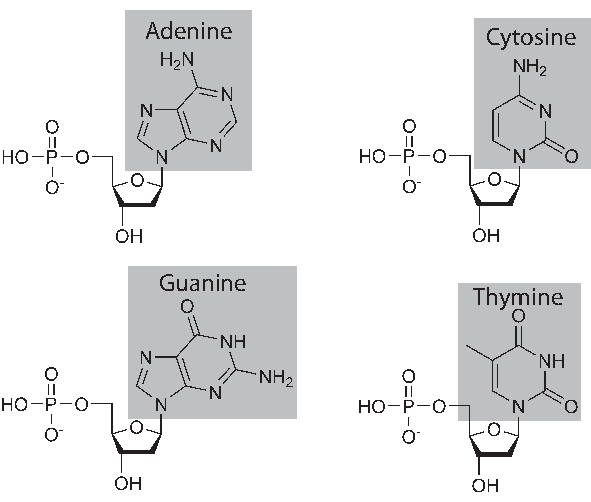
\includegraphics[width=\smallfigure]{\FIGPATH/Figures_Intro/nucleotides}
\caption[Nucleotides, the elementary subunits of DNA.]{
\label{fig:nucleotides} The four different nucleotides of DNA: Each nucleotide
consists of a phosphate group, the sugar desoxyribose and one of the bases adenine, 
cytosine, guanine or thymine.
 Source of images: Wikipedia.}
\end{figure}

Single stranded DNA (ssDNA) alone is not suitable as a storage medium for hereditary information 
because single phosphate bonds are not stable enough and a damaged single strand is hard to repair without a backup copy.
\nomenclature{ssDNA}{Single stranded DNA}
\nomenclature{dsDNA}{Double stranded DNA}
Both problems are solved elegantly by the ability of ssDNA to pair with a 
\emph{complementary} strand. The geometry of the bases 
adenine and thymine is such that they can form two hydrogen bonds, whereas
cytosine and guanine interact via three hydrogen bonds, cf.~\FIG{DNA_structure}. 
The interaction between these bases occurs only, if they are aligned in opposite 
polarity. Therefore a DNA strand binds 
selectively to a strand, the sequence of which is the complementary sequence in opposite
order. After base pairing, the double stranded DNA (dsDNA) winds into a double helix, which brings consecutive
base pairs closer together and shortens the duplex from 0.7~nm per base in single strand
to 0.34~nm in double strand. The double helix has an diameter of approximately 2~nm and a
helical pitch of about 10.5~bp or 3.5~nm. By base pair stacking, water
is driven out of the space between base pairs and the carbon rings of bases align, which 
is the major contribution to the DNA binding free energy. The DNA double helix is not completely
symmetric, meaning the two bases of a base pair do not form an angle of 180${}^\circ$. 
Thereby, dsDNA has a major and a minor groove, as illustrated in \FIG{DNA_structure}b.
\nomenclature{Stacking interactions}{Consecutive base pairs in dsDNA stack on top of each other
and thereby drive water out of the inter-base region. These stacking interaction are a major 
contribution to the DNA binding free energy\refpage}%

In contrast to ssDNA, damage to dsDNA is easy to repair. 
The complementary strands can serve as a template for reconstruction of a damaged strand
and for replication of the molecules. The stability of dsDNA and its potential to be repaired
enable cells to maintain genomes as long as $10^{10}$ nucleotides, resulting in molecules of 
macroscopic length.
\begin{figure}
\centering
  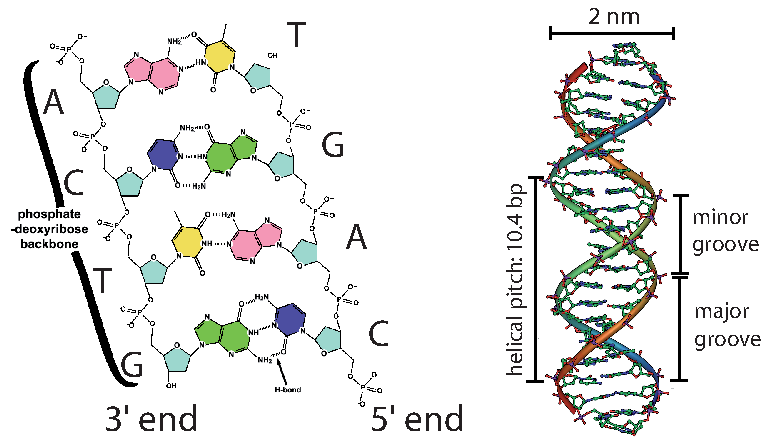
\includegraphics[width=0.7\columnwidth]{\FIGPATH/Figures_Intro/DNA_structure}
\caption[Structure of dsDNA]{\label{fig:DNA_structure} Left: Two oppositely aligned DNA strands
bind specifically to each other if their sequences are complementary, i.e. if
each base \basepair{A} faces a \basepair{T} and each base \basepair{G} faces a \basepair{C}. Hydrogen bonds
between bases are indicated by dashed lines. 
%Two complementary DNA strands thus form a ladder-like structure
%where the sugar-phosphate backbones form the stiles and the base pairs the rungs.
Right: The ladder-like structure compactifies further by winding into a double helix.
The pitch of the double helix 3.5~nm, which corresponds to $\approx 10.5$~bps. 
Since base pairs are not perfectly straight the helix displays a major and a minor groove.   
%The double helix is stabilized by stacking interactions between $\pi$-bonds of consecutivebases. 
Source of images: Wikipedia.}
\end{figure}


\section{Thermodynamics of DNA}
In the previous section we discussed how the chemical architecture of DNA makes it an
ideal carrier of genetic information. We will now turn to thermodynamic properties
of DNA which have implications for the ability of cells to read the sequence information from the DNA. 
Efficient information read out is possible only when the double helix is opened and the unpaired bases are exposed. Hence, the cell has to separate dsDNA locally into single strands at ambient temperature.
How this can be achieved is mainly determined by binding affinity of the two strands and their 
fluctuation properties, which therefore have been studied extensively, both
experimentally and theoretically. 

The basic ingredients to DNA thermodynamics are the free energy contributions of base pairing
and stacking interactions. Using these parameters, the properties of short 
molecules can be well understood with simple two state models. 
Subsequently we discuss the melting behavior of long molecules and calculate the 
partition sum of a dsDNA molecule within the framework of the Poland-Scheraga model.
%When studying repetitive DNA in chapter \ref{sec:DNA_sliding} we will generalize the 
%Poland-Scheraga model to incorporate non-native base pairings. 

\subsection{Binding free energies of double stranded DNA}
The dominant contributions to the binding free energy of double stranded DNA are
H-bonds between bases in Watson-Crick base pairs and the stacking
interaction between subsequent base pairs. The binding of the two strands goes along
with a significant reduction in entropy, since two floppy single strands are forced into 
a much more rigid double stranded conformation. 
Assuming constant specific heat $c_p$, the free energy of a particular structure is given 
by
\begin{equation}
\label{eq:DNA_free_energy}
\Delta G = \Delta H -T\Delta S,
\end{equation}
where enthalpies, entropies and free energies are measured with respect to the dissociated
case. To a good approximation, $\Delta H$ and $\Delta S$ can be calculated as sums from 
contributions of consecutive base pairs, such as \basepair{AG/CT}. Additional free energy contributions 
stem from penalties for mismatches and loops or the lack of stacking interactions at the first and last
base pair, often called initiation  and termination costs.
\begin{equation}
\label{eq:DNA_free_energy}
\Delta G = \Delta G_{init} +\sum_{basepairs} \Delta G_{bp} + \sum_{loops} \Delta G_{loop}+\sum_{mismatches} \Delta G_{mm}+\Delta G_{term}.
\end{equation}
Many of the parameters have been carefully measured and are reviewed by 
\citeauthor{SantaLucia_PNAS_98} in \cite{SantaLucia_PNAS_98} and 
\cite{SantaLucia_AnnRevBioPhys_04}. While the precise binding energies depend on at least two consecutive base pairs, a good
rule of thumb is that a \basepair{CG} base pair contributes approximately $3\kT$ and an \basepair{AT} pair
about $2\kT$ at physiological salt concentrations. The penalty for initiating a loop, that is interrupting base pair stacking, is typically between $3$ and $10\kT$. 
%In contrast to the base pairing contributions, the penalties to initiate 
%and terminate the helix are length independent and are hence of particular importance for short molecules (up to 30 bps). The
%shorter a molecule, the lower its melting temperature. 
Extrapolation formulas of the parameters to 
different salt concentrations are also available \cite{SantaLucia_AnnRevBioPhys_04}. The complete set of 
parameters has been fed into software packages that predict melting temperatures and
plausible secondary structures of short DNA oligonucleotides, see for example \cite{Zuker_NAR_03}.

\paragraph{Two-state models.} 
Short DNA oligonucleotides occur in essentially two different states. The two strands are either
dissociated and float freely in solution, or the two strands are bound in their most stable binding 
configuration since any suboptimal base pairing is unstable. 
For such molecules, it is particularly easy to predict their melting temperature. 
%The free energy difference of the double 
%stranded state compared to the dissociated state is given by
%\begin{equation}
%\label{eq:DNA_free_energy_incl_conc}
%\Delta G = \Delta H -T\Delta S,
%\end{equation}
%where $\Delta H$ is the binding enthalpy and $\Delta S$ the reduction in entropy. 
The melting temperature $\Tm$ is commonly defined as the temperature where half of the 
single strands are part of duplexes. Setting $\Delta G$ in \EQ{DNA_free_energy} to zero and accounting for the 
 total concentration of DNA strands $c_T$, one finds \cite{SantaLucia_PNAS_98}
\begin{equation}
\label{eq:DNA_two_state_Tm}
\Tm = \Delta H/(\Delta S+R \ln c_T),
\end{equation}
where the gas constant $R=1.9872\frac{\mathrm{cal}}{\mathrm{K\cdot mol}}$.
Due to significant contributions from terminal ends, the melting temperature of short 
molecules strongly depends on the length. At larger length (above 30 base pairs), the melting temperature
mainly depends on the bulk binding energy and hence on the \basepair{CG} content of the sequence. 
Melting temperatures range from $20\Celsius$ for very short (5 base pairs) sequences 
to $90\Celsius$ for long \basepair{CG}-rich molecules.

\subsection{\label{sec:DNA_melting}Denaturation of long DNA molecules}
The assumption that two DNA strands are either firmly bound in the most stable state,
or completely dissociated is not justified for long sequences. Long sequences might have 
regions with different \basepair{CG}-content that melt at different temperatures. Even 
homogenous molecules will once in a while open their double stranded structure locally and 
form denatured bubbles as illustrated in \FIG{DNA_melting_experiment}. Two-state models are therefore not suitable for long molecules, but 
many different configurations  including partly melted patches contribute significantly. The most
important experimentally accessible quantity is the degree of base pairing of the DNA strands, 
which can be monitored 
by the absorption of UV light. Unpaired bases absorb UV light more efficiently than bases 
stacked in the double helical conformation and any change in the absorption coefficient can be
directly related to the degree of base pairing $\Theta(T)$ between the two strands \cite{Wartell_PhysRep_85}. 
If the local \basepair{CG}-content is constant along the molecule, the derivative 
$-\frac{d \Theta(T)}{d T}$ of the fraction of bound base pairs $\Theta$ 
has a single peak. However, the \basepair{CG}-content of DNA varies considerably along the genome\footnote{
There are differences in \basepair{CG}-content between coding and non-regions, 
as well as between incorporated viral DNA and proper DNA.}. 
In this case, the differential melting curve has many peaks corresponding to
different regions of the DNA that melt at different temperatures. A typical melting curve is shown 
in \FIG{DNA_melting_experiment}.
\begin{figure}
\centering
  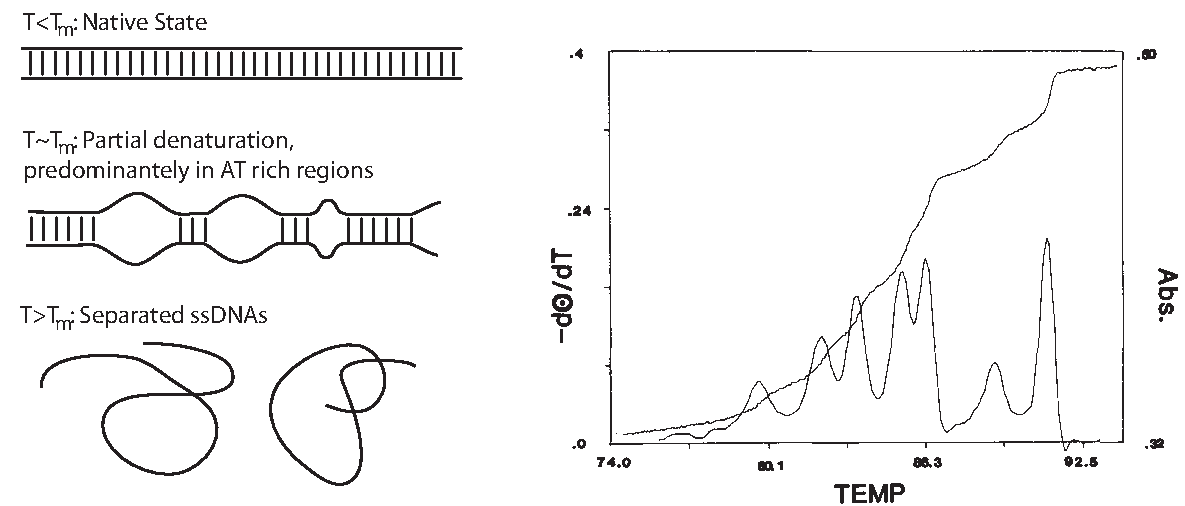
\includegraphics[width=\largefigure]{\FIGPATH/Figures_Intro/DNA_melting_experiment}
\caption[DNA melting curve.]{
\label{fig:DNA_melting_experiment} 
Left: With increasing temperature the double stranded structure of DNA is interrupted by 
denatured loops and the two strands eventually separate. \basepair{AT} rich regions tend to denature
at lower temperatures due to their smaller binding free energy. Left: The UV absorbance and the negative 
differential of the fraction of base pairs vs. temperature, see main text.
%The differential melting curve has multiple peaks, corresponding to different stretches of DNA that 
%denature at different temperatures.
Reproduced from \cite{Wartell_PhysRep_85}.}
\end{figure}

Attempts to describe the melting transition of DNA theoretically date back to the late 1950s and
resulted in a class of models that are now commonly referred to as Poland-Scheraga models 
\nomenclature{PS-models}{Poland-Scheraga models. A class of models for base pairing configurations of 
dsDNA\refpage}%
\cite{Zimm_JChemPhys_59, Zimm_JChemPhys_60, Poland_JChemPhys_66a, Poland_JChemPhys_66b} or Ising
type models. These models describe a particular configuration of the DNA by the set of base pairs formed. In general, 
base pairs can be formed between any two complementary bases on different strands 
as wells as within one strand, that folds back onto itself. The latter is particularly important for RNA, 
but is rarely relevant for two complementary DNA strands since a high 
degree of self complementarity within a single strand is unlikely. 
%It is further assumed that base pairs do not cross, \emph{i.e.}~denatured loops and double helical stems
%alternate along the molecule.
Poland-Scheraga models are usually restricted to native base pairs, \emph{i.e.}~only base pairs
that are present in the ground state are allowed. The restriction to native base pairs is a good approximation, since
stable base pairing requires several consecutive base pairs and the chance of finding two non-native complementary 
stretches that are several base pairs long is slim. A convenient way to denote a base pairing configuration 
of dsDNA of length $N$ is by an ordered subset of the integers $\cS={i_1, \ldots, i_m}\subset[1,\ldots, N]$, 
which corresponds to the base pairs present in the DNA duplex.
Since we are not interested in reproducing experimental data as faithfully as possible, but rather
seek generic explanations to general features of DNA denaturation, it is reasonable to simplify the free energy 
model. In the following, we assume that stacking interactions do not depend on the base pair type
and include them through a cost $\Eini^{0}$ for initiating a loop. Furthermore, we assume that 
the loop penalty is independent of the bases in the loop and only depends on the loop size.  
%\begin{figure}
%\centering
%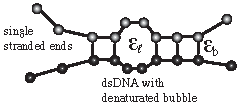
\includegraphics[width=\smallfigure]{\FIGPATH/Figures_Intro/PS_model}
%\caption[Poland-Scheraga model of base pairing.]{
%\label{fig:PS_model}Base pairing model of Poland-Scherage type. A base pairing
%free energy $\eps$ is assigned to each base pair of the sequence and a loop penalty
%to each internal loop, which interrupts the stacking of consecutive base pairs. Obviously, 
%the base pairing energy depends on the type of base pair (C-G or A-T) and the loop penalty
%might depend on the length of the loop and the sequence composition.}
%\end{figure}
The free energy model for a DNA configuration then simplifies to% (comp. \FIG{PS_model})
\begin{equation}
\label{eq:dna_melting_energy}
G[\cS]=-\sum_{i\in \cS} \eps(i) + \sum_{loops} \Eini(n_l),
\end{equation}
where $\eps(i)$ is the binding energy of base $i$ and $\Eini(n)$ is the free energy cost of a loop of size $n$.
However, even with this simple free energy model the explicit summation of all configurations 
is infeasible, since their number increases exponentially with the length.
Fortunately, there is a much more clever way to calculate the partition sum. Any allowed 
base pairing configuration is a sequence of double stranded stems and denatured
loops. Furthermore, the free energy of a particular configuration is a sum of local contributions 
from base pairs and loops. These properties allow the calculation of the partition function using recursion relations.
Let $Z_n$ be the partition function of a dsDNA molecule of length $n$, 
where the first and the last base pair are formed. $Z_n$ obeys the recursion relation
\begin{equation}
\label{eq:PS-recurrence}
Z_n=e^{\frac{\eps(n)}{\kT}} Z_{n-1}+\sum_{m=1}^{n-2}e^{\frac{\eps(n)-\Eini(m)}{\kT}} Z_{n-m-1},
\end{equation}
where the first term includes any structure that can be obtained by adding base pair $n$ to any configuration
in $Z_{n-1}$ and the sum includes all structures that are obtained when adding the base pair $n$
followed by a loop of size $m$ to any structure in $Z_{n-m-1}$.
%\begin{figure}
%\centering
%  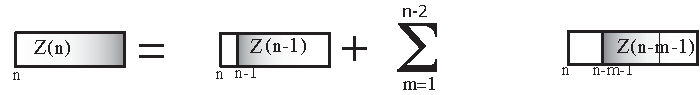
\includegraphics[width=\smallfigure]{\FIGPATH/Figures_Intro/recursion_relation}
%\caption[Recurrence relation for the partition sum.]{
%\label{fig:recursion_relation} 
%Recurrence relation for $Z_n$.
%}
%\end{figure}
This recursion relation allows the calculation of the partition sum of arbitrary sequences of length $N$
in $\mathcal{O}(N^{2})$ steps. Similar recursion relations have been used to study the statistical physics
of RNA strands that fold back onto themselves \cite{Bundschuh_PRL_99, Flamm_RNA_00}.

\paragraph{The length dependence of the loop cost.}
When describing a dsDNA molecule by its set of base pairs it is implicitly assumed, that
all other degrees of freedom, \emph{e.g.}~the conformation of single stranded ends or denatured loops 
equilibrate rapidly compared to major rearrangements in the base pairing patterns. 
This results in a subtle dependence of the free energy of a loop on its length. Single stranded
DNA is rather flexible and changes its orientations typically every 2 to 3 base pairs, see \SEC{stretching_ssDNA}.
The possible conformations of ssDNA can therefore be mapped to the configurations of 
a random walk\footnote{Excluded volume effects of free single strand are not essential for the 
denaturation transition.}. The number of random walks increases as $\sim s^{n}$ with its length $n$. 
For ssDNA, $s$ has to be chosen such that $\ln s$ is the decrease in entropy when 
a single stranded monomer is forced into dsDNA. 
A denatured bubble in a dsDNA can also be described by a random walk, however, subject
to the constraint that the random walk forms a closed loop. This reduces the number of 
allowed configurations by a factor $n^{-c}$ giving rise to a loop penalty of entropic
origin of the form $c\ln n$ \cite{deGennes_79}. For ordinary random walks in $d$ dimensions $c$ has 
the value $d/2$. When self-avoidance is included, $c$ is given by $d$ times the Flory exponent $\nu$. 
At first sight this logarithmic correction to entropy appears to be of minor importance, but it is responsible
for a genuine denaturation transition in Poland-Scheraga models (see below). In particular,
a discontinuous transition requires $c\!>\!2$.
\citeauthor{Kafri_PRL_00} claim that $c$ is indeed larger than 2 when mutual 
excluded volume effects of different loops are taken into account \cite{Kafri_PRL_00}.  
In a nutshell the argumentation is
as follows: The denatured loops in a DNA molecule are not independent self-avoiding
polymer loops, but are linked by the double stranded stem to form a polymer network.
Excluded volume effects in a connected polymer network are stronger than for non-interacting loops, resulting
in a higher value of the exponent $c$. \citeauthor{Kafri_PRL_00} calculated a value of $c=2.15$ for DNA
denaturation, resulting in a discontinuous transition \cite{Kafri_EPJE_02}. 
However, the applicability of the scaling theory of polymer networks to DNA has been 
questioned \cite{Hanke_PRL_03, Kafri_PRLcomment_03}. The objection is, that denatured loops
are rare and far apart such that their interaction should be negligible. The rigid double stranded 
stems are essentially one dimensional objects, which are irrelevant for scaling. In any case, 
corrections to the loop exponent will only become important when studying DNA melting 
using extremely long molecules with very homogenous sequences.
For now, we treat $c$ as a variable and use a loop initiation cost of the form
\begin{equation}
\label{eq:loopcost}
\Eini(n)=\Eini^{0} -n\ln s + c\ln n,
\end{equation}
where $\Eini^{0}$ is a constant loop initiation cost due to the loss of base pair stacking
when a loop is formed. 

\subsection{\label{sec:DNA_melting_homo}DNA melting of homogenous sequences}
While the recursion relations are indispensable when studying the thermodynamics of
a particular sequence, they do not provide insight into the universal properties of DNA melting. 
To this end, we now demonstrate how the partition sum can be calculated in closed
form if the binding energy per base is the same for every base.  This might appear
to be a very restrictive and unrealistic assumption. However, we can coarse grain our 
description even further and lump a small number of bases together and treat them 
as a single entity. Given the sequence is random, the relative fluctuations of the 
binding energy of such ``super bases" become small. At the same time, each super base is likely to have a unique binding partner,
as assumed when choosing the set of allowed configurations. 
The assumption made is thus not that restrictive and the homogenous Poland-Scheraga 
model is adequate to study the melting transition\footnote{Obviously, this assumption
breaks down when macroscopic regions differ in \basepair{CG} content.
%, such as coding and non-coding DNA
}.

%If the loop penalty is independent of the loop size, the PS model is equivalent to an Ising model in
%one dimension. 
Poland-Scheraga models are essentially one-dimensional, similar to an Ising model.
It is well known, that one dimensional models do not exhibit 
genuine phase transitions. This fact is in conflict with the observed melting behavior of DNA and the 
apparent contradiction troubled (theoretical) physicists a while.
A genuine melting transition is only obtained if the proper dependence of
the loop cost on the loop length is included in the model.
The logarithmic term in \EQ{loopcost} introduces an effective long range interaction, that gives rise to  
an order-disorder phase transition in such one dimensional models \cite{Fisher_JChemPhys_66}.
The detailed thermodynamics of DNA was worked out by \citeauthor{Poland_JChemPhys_66a}
in the publications \cite{Poland_JChemPhys_66a,Poland_JChemPhys_66b} and later 
summarized in their book \cite{Poland_Scheraga_70}. We will now briefly summarize
the statistical physics of homogenous DNA following  \citeauthor{Poland_JChemPhys_66a}.
For a homogenous DNA molecule the recursion relation \EQ{PS-recurrence} simplifies to
\begin{equation}
\label{eq:PS_partsum}
Z_{n} = q Z_{n-1}+\sum_{m=1}^{n-2}\frac{qg^{2}s^{2m}}{m^{c}} Z_{n-m-1},
\end{equation}
where $q=e^{\frac{\eps}{\kT}}$, $g^{2}=e^{-\frac{\Eini^{0}}{\kT}}$ and the starting value of the recursion is 
set to $Z_1=q$. This recursion relation can be solved by $z$-transformation. The $z$-transform of
$Z_n$ is defined as $\Zh(z)=\sum_{n=0}^{\infty} Z_n z^{n}$ and is also known as generating function 
or discrete Laplace transform. Multiplying both sides of \EQ{PS_partsum} by $z^{n}$ and summing 
over $n$ yields after some algebra
\begin{equation}
\label{eq:PS_z_transform}
\frac{\Zh(z)-qz}{z} = q\Zh(z)+qg^{2}\Phi_c(zs^{2})\Zh(z),
\end{equation}
where $\Phi_c(z)=\sum_{n=1}^{\infty}\frac{z^{n}}{n^{c}}$ is the polylogarithm. \EQ{PS_z_transform} 
is readily solved for $\Zh(z)$
\begin{equation}
\label{eq:PS_Zh}
\Zh(z) = \sum_{n=0}^{\infty} Z_n z^{n}=\frac{qz}{1-qz-qg^{2}z\Phi_c(zs^{2})}.
\end{equation}
This $z$-transformed partition sum is nothing but the grand-canonical partition sum of a DNA
molecule coupled to a fictive nucleotide reservoir with fugacity $z$. 
The original partition sum of a molecule of length $N$ can now be recovered from $\Zh(z)$ by 
contour integration around the origin of the complex plane.
\begin{equation}
\label{eq:contour_integral}
Z_N = \frac{1}{2\pi i}\oint dz\: \frac{\Zh(z)}{z^{N+1}}=\frac{1}{2\pi i}\oint dz\: \sum_{n=1}^{\infty}\frac{Z_n}{z^{N-n+1}}
\end{equation}
The function $\Zh(z)$ is analytic everywhere, except on $[s^{-2}, \infty[$ and possibly at 
isolated singularities, \emph{i.e.}~zeroes of the denominator of \EQ{PS_Zh}. 
Having identified the singularities and branch-cuts, the contour integral can be evaluated by
calculating the residuals and the integral encircling the branch-cut, as illustrated in \FIG{contour_integral}.
A graphical solutions for zeroes of the denominator for different values of $c$ are given in \FIG{contour_integral}.
At low temperatures, that is large $q$, the denominator has a real root $\zc$.  
If $c>1$, this root merges with the branch-cut at some critical temperature and does not exist in
the high temperature regime.
\begin{figure}
\centering
  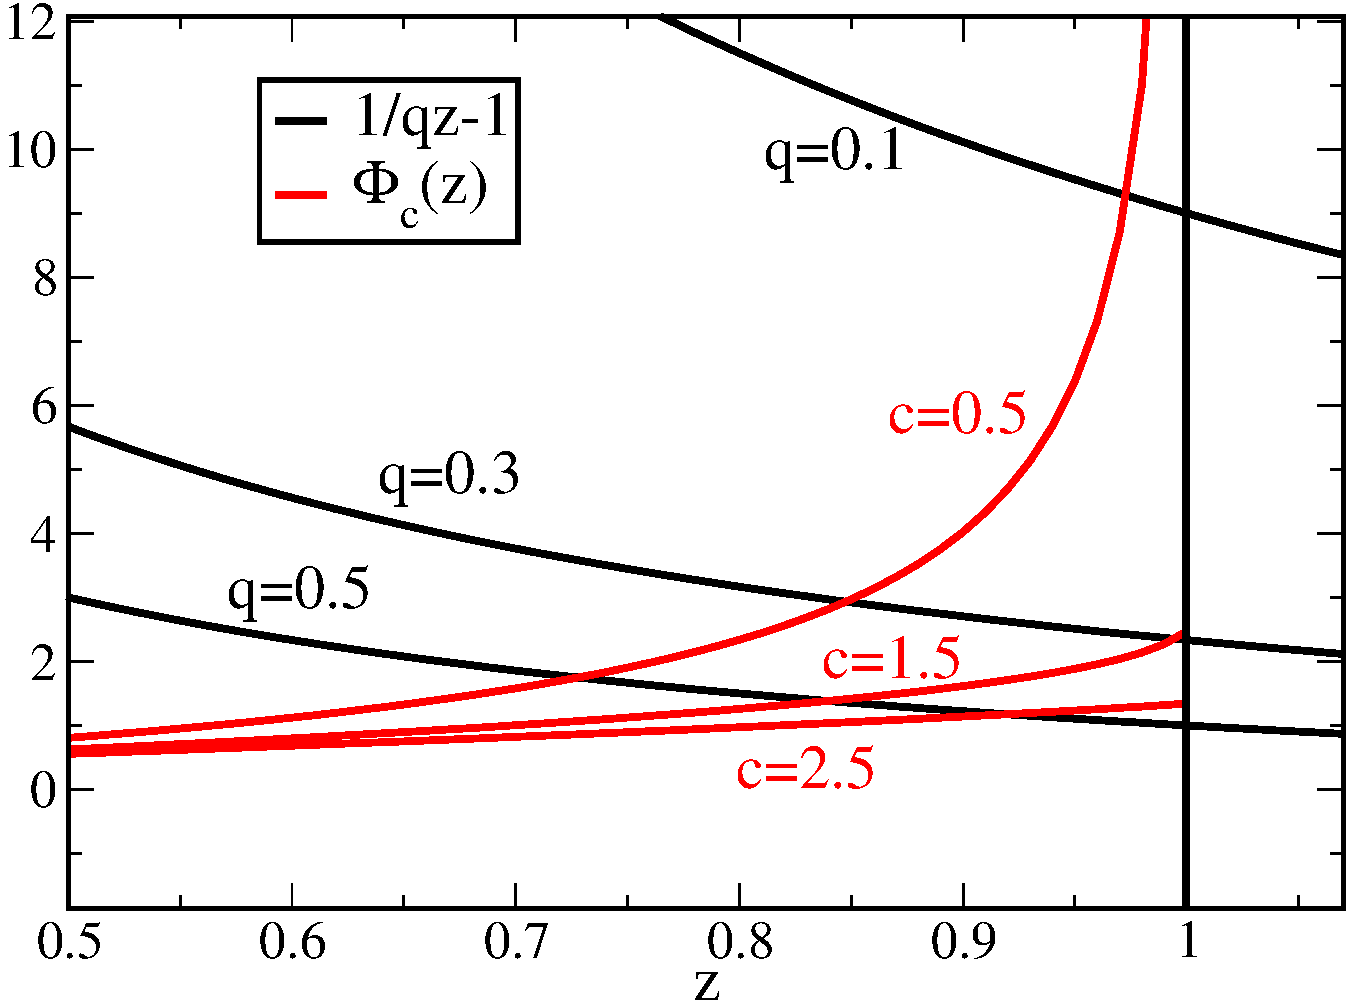
\includegraphics[width=\halffigure]{\FIGPATH/Figures_Intro/graphical_sol}
  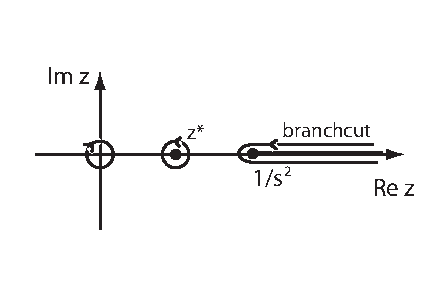
\includegraphics[width=\halffigure]{\FIGPATH/Figures_Intro/contour_integral}
\caption[Contour integration in the fugacity plane.]{
\label{fig:contour_integral} 
Left: Zeros $\zc$ of the denominator of \EQ{PS_Zh} are given by the
intersections of $g\Phi_c(zs^{2})$ and $q^{-1}z^{-1}-1$ ($g$ and $s$ are set to 1 for simplicity).
%If $c<1$, there is a solution $\zc$ for every $q=e^{-\frac{\eps}{\kT}}$ and no melting transition exists (see main text).
Right: Contour integration in the fugacity plane. The contour integral around the origin is the sum 
of the residue at $z=\zc$ and the integral encircling the branch cut. For large $N$, the integral
is dominated by the residue.
}
\end{figure}
The partition function of a DNA molecule of length $N$ is therefore of the form 
\begin{equation}
\label{eq:residues}
Z_N =\frac{Res(\Zh(z), \zc)}{\zc^{N+1}} + As^{2N} \quad \mathrm{or} \quad Z_N =As^{2N},
\end{equation}
depending on whether the root $\zc$ exists or not. 
If $\zc$ exists, the fraction $\Theta$ of base pairs present in the
structure is given by the logarithmic derivative of $\ln Z_N$ with respect to $q$
%WOLFRAM ASKED FOR ADDITIONAL HINTS
\begin{equation}
\label{eq:fraction_basepairs}
\Theta=\frac{1}{N}\frac{\partial \ln Z_N}{\partial \ln q}= -\frac{\partial \zc}{\partial \ln q}.
\end{equation}
If the isolated singularity does not exist $Z_N$ does not depend on $q$ and $\Theta$ vanishes. 
The existence of $\zc$ is therefore connected to the phase where 
the two strands are bound and the temperature at which $\zc$ ceases to exist corresponds to the 
melting temperature $\Tm$. 
The order of the melting transition is 
determined by the value of the loop closure exponent $c$ \cite{Poland_JChemPhys_66b,Kafri_EPJE_02}: 
If $c\leq 1$, $\Phi_c(z)$ diverges as $z\to 1$, hence there is always a solution $\zc$ and no melting transition
exists. If $1\!<\!c\!\leq\!2$, $\Phi_c(z)$ remains finite as $z\to 1$ but approaches its limiting value
with infinite slope, resulting in a melting transition where $\Theta$ approaches zero as $T\to \Tm$ and the 
melting transition is continuous.
If $c>2$, $\Phi_c(z)$ tends to its limiting value with finite slope and $\Theta$ drops from
a finite value to zero at $T=\Tm$, giving rise to a first order melting transition.
Experimental melting curves of DNA are very steep, \emph{i.e.}~the fraction of bound bases vanishes 
very rapidly, and denaturation appears to be a first order transition. The additional contributions
to $c$ from loop interactions might therefore be relevant to reconcile the Poland-Scheraga models with experimental data. 
Available experimental data has been reexamined using $c=2.15$ instead of $c=3\nu\approx 1.8$, resulting in a smaller
estimate of the effective loop initiation cost \cite{Blossey_PRE_03}.

%REFER TO THE VALUE OF C

\section{\label{sec:DNA_mechanical_properties}Mechanical properties of DNA}
So far, we discussed the chemical and thermodynamic properties of DNA and 
neglected the organization of DNA in space. A typical human
chromosome is $10^{8}$~bp long, corresponding to a string of 3~cm in length. 
Forty-six of these strings have to fit into the cell's nucleus, which is only several micrometers
in diameter. Packaging and compactifying DNA is thus a nontrivial issue to cells, especially since
they have to keep their genome, or at least the relevant parts, accessible. This problem 
is addressed in the second part of this thesis. Obviously, the mechanical properties 
of DNA play an important role in DNA compactification and the dynamics of compactified DNA. 
During the last 15 years, it has become possible to study the mechanical properties of DNA by
 manipulating single molecules and measuring
their response to pico Newton forces. These single molecule force spectroscopy techniques provided
unprecedented insight into the static and dynamic properties of biological macromolecules 
and even allow to study cellular machinery such as polymerases or topoisomerases 
life on stage. The dynamics of repetitive DNA sequences
has also been studied using such techniques, which will be discussed in chapter \ref{sec:DNA_sliding}.
I will therefore give a brief overview
over such techniques and then discuss the mechanical properties of DNA.

\subsection{\label{sec:force_spectroscopy}Single molecule force spectroscopy}
At the molecular level, biological processes involve energy differences of the order of the thermal energy
$1\kT\approx 4\,pN\,nm$ and length scales on the order of nano meters.
To probe biological macromolecules mechanically, 
instrumentation is needed that is capable of applying forces in the pico Newton 
regime and measure distance with nano meter resolution. By now, a variety of different
techniques are available to achieve this feat and I will briefly discuss their basic mechanism
as well as their advantages and drawbacks. Atomic force microscopy is discussed in a little
more detail, since the slippage of repetitive DNA was detected using this technique
(see also \SEC{DNA_slippage_experiments}). For comprehensive reviews of the 
different techniques see for example \cite{Merkel_PhysRep_01, Bustamante_NMCB_00,Clausen-Schaumann_CurrOpChemBio_00}.

\paragraph{Optical tweezers.} 
When an object with an optical density higher than the surrounding  media is placed
in a non-uniform electric field, it feels a force towards the stronger field. This effect is exploited
in optical traps, where a small spherical bead is held in a laser focus. As soon as the bead is 
no longer centered in the focus, it experiences a restoring force. Although the explanation illustrated
in \FIG{force_spectroscopy} is not exactly applicable to beads of sizes of the order of a micrometer, it
conveys the essence of the method. The laser light is refracted by the bead and thereby transmits
momentum to the bead. If the bead is not centered, the laser intensity on the two sides of the bead
are not equal and hence the transmitted momenta do not balance, resulting in a net force towards
the focus. To study the response of a system to mechanical force, it is attached to the
bead and the exerted force can be determined by measuring the deviation of the bead from the 
trap center.  Interferometric methods allow to determine the bead position to nm resolution,
which for typical trap stiffnesses results in force resolution of pN and below.
The maximal forces optical traps can apply depend on the bead size and are in the range of 20 to 150pN.
One important application of optical tweezers has been the unzipping of single DNA molecules
\cite{Bockelmann_BiophysJ_02}, which is discussed in more detail below in \SEC{DNA_unzipping}. 
The motion of single processive molecular motors has also been studied using optical tweezers \cite{Clemen_BioPhysJ_05}.

\begin{figure}
\centering
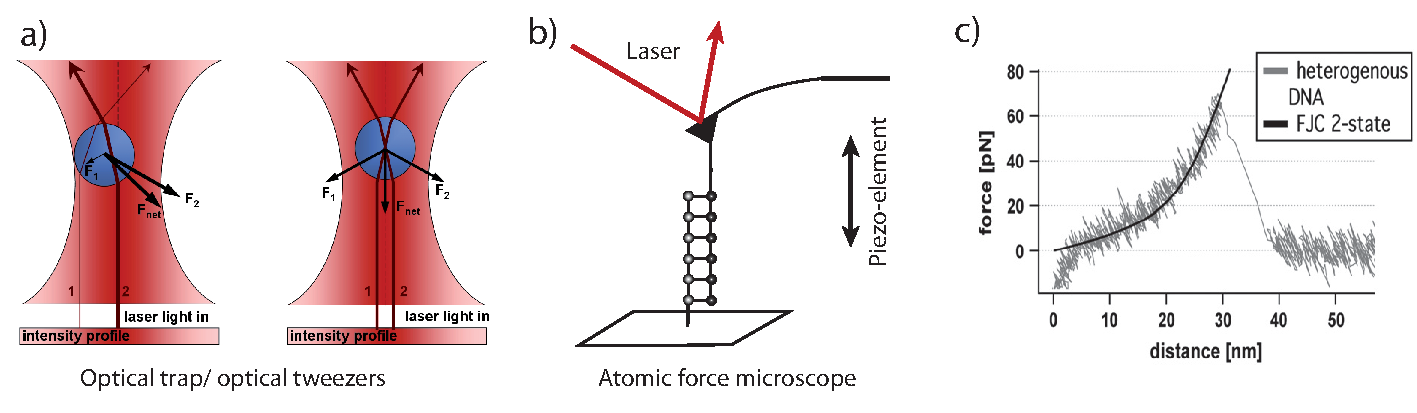
\includegraphics[width=\largefigure]{\FIGPATH/Figures_intro/force_spectroscopy}
\caption[Sketch of an optical trap and an AFM.]{\label{fig:force_spectroscopy}
Part a) Ray optics explanation of an optical trap. Image source: Wikipedia. b) Sketch of an AFM in a single molecule experiment. The different parts are extremely out of scale. c) A typical force-extension curve recorded with an AFM 
(taken from \REF{Kuehner_BiophysJ_07}).
}
\end{figure}

\paragraph{Magnetic tweezers.}
Similar to optical tweezers, magnetic tweezers exploit the fact that magnetic dipoles are attracted to high 
field regions and therefore experience a force in a gradient field. In addition to force, magnetic
fields exert torque on permanent magnetic dipoles. This opens up the possibility to twist biomolecules
by rotating the magnet that generates the field. The position of the beads can be detected using 
similar interferometric techniques as for optical tweezers, reaching nm resolution. The force 
can be sensitively controlled through the field gradient and forces as small as 10~fN can be applied. 
Magnetic tweezers have been used to study the stretching response of supercoiled DNA \cite{Strick_Science_96}
and to observe topoisomerases, the enzymes that disentangle DNA, in action \cite{Strick_Nature_00}.

\paragraph{Biomembrane force probes.}
Yet another technique of measuring small forces are biomembrane force probes. 
Small lipid vesicles or red blood cells are partially sucked into a micropipette to establish a 
well controlled tension of the vesicle membrane. The system to be studied is attached 
to the other end of the vesicle and pulled away. The deformation of the vesicle
can be related to the force applied to the sample. This technique has been used
for measuring the binding strength and kinetics of receptor-ligand systems \cite{Merkel_Nature_99}. 

\paragraph{Atomic force microscope.}
\nomenclature{AFM}{Atomic force microscope\refpage}
While optical and magnetic techniques excel at small forces with exquisite resolution, the realm 
of the atomic force microscope (AFM) are forces above 5pN. Among all force spectroscopy techniques,
the AFM has by far the greatest spatial resolution, which can be as good as the diameter of an atom.
Historically, AFMs were invented to map surfaces at atomic resolution, and only later became important tools
to study mechanical properties of biological macromolecules or molecular complexes. 
An AFM used for force spectroscopy consists of a tiny solid state cantilever with an even tinier tip. The substrate surface is mounted 
onto a piezo element which allows to move the sample with respect to the cantilever with extremely 
high precision. A force exerted on the cantilever will cause a slight bend in the cantilever. 
This minute deflection can be measured by shining a laser beam onto the reflective upper side of the 
cantilever, as sketched in \FIG{force_spectroscopy}. 
A deflection of the cantilever changes 
the reflection angle of the beam, which in turn can be sensitively detected by a split photodiode.
Since control and detection is done by fast electronic devices, 
the bandwidth of AFM measurements can be as high as 100kHz and
is limited by the viscous damping of the cantilever.

The substrate and the cantilever have to be prepared such that upon bringing the cantilever
in contact with the substrate, the sample attaches to both, the 
substrate and the cantilever. Often, the connection to the cantilever and substrate is 
established via well characterized and chemically functionalized linker molecules. 
Using linker molecules increases the distance of the sample from the surface and thereby reduces
surfaces effects. The sample density has to be chosen such that a single contact
between cantilever and substrate is more probable than multiple linkages. The substrate surface is then
retracted and the force is measured as a function of extension. Depending on the question 
to address, the force extension relation or the dependence of rupture forces on retract speed 
are informative quantities. 

\subsection{\label{sec:stretching_dsDNA}Stretching double stranded DNA}
%Among the first biomolecular applications of force spectroscopy was stretching dsDNA. 
%By now, the mechanical properties of DNA in different force and length regimes are fairly well understood.
\nomenclature{WLC}{Worm-like chain\refpage}%
On a microscopic scale, dsDNA is a very stiff polymer and thermal forces bend DNA
only on length scales long compared to the helical pitch  or even individual base pairs. 
To a good approximation, the DNA bendability is continuously distributed along the DNA
and the typical curvature radius is large compared to molecular dimensions. 
On the other hand, up to forces of about 50pN, dsDNA is virtually inextensible. 
Ignoring excluded volume effects the equilibrium conformations of DNA are therefore 
well described by the ensemble of inextensible
contour lines with a linear bending stiffness, a model commonly referred to as \emph{worm-like-chain
model} (WLC) \cite{Saito_JPSJap_66, Kratky_Porod_49}. The energy of a particular contour $\mathbf{r}(s)$ with a force $\mathbf{f}$ pulling
the endpoints apart is given by
\begin{equation}
\label{eq:WLC_energy}
E=\frac{\kappa}{2} \int_0^{L} ds\; \mathbf{t}'(s)^{2} -\mathbf{f}\cdot(\mathbf{r}(L)-\mathbf{r}(0)),
\end{equation}
where $\kappa$ is the bending stiffness and $\mathbf{t}'(s)$ denotes the derivative of the 
tangent vector with respect to the arclength $s$. To calculate the equilibrium properties of 
such a chain immersed in a heat bath, one would have to calculate the integral over all
possible paths $\mathbf{r}(s)$, which in general is infeasible. Some quantities, however, can 
be calculated exactly. In the absence of force, the 
most important exactly known quantity is the tangent correlation 
function at different points of the contour. 
\begin{equation}
\label{eq:WLC_tangentcorr}
\langle \mathbf{t}(s)\cdot\mathbf{t}(s')\rangle=e^{-\frac{|s-s'|}{\lp}},
\end{equation}
where $\lp=\frac{\kappa}{\kT}$ is called the persistence length. 
%Other exactly known quantities
%are the mean end-to-end distance or the radius of gyration \cite{WLC_lit}. Introduction of 
%self-avoidance renders the problem completely intractable.	
The persistence length is the length scale at which the correlations of different parts of the chain
decay and a molecule is considered flexible, if its total length is large compared to $\lp$. 
Conversely, a chain several times smaller than the persistence length is typically straight.
The persistence length of double stranded DNA under physiological conditions is $\lp=50\nm$.

\paragraph{Short molecules.}
Polymers that are short compared to the persistence length are often referred to as \emph{semi-flexible}.
The typical contours of these polymers are deviations from a straight line. If the straight
contour is the $z$-axis, the contour can parameterized by two single valued functions
$x(z)$ and $y(z)$. Furthermore, longitudinal contraction is only of second order, such that we can 
identify the arclength with $z$. Within this weakly bending approximation, the equation of motion of the
polymer is given by \cite{Barkley_JChemPhys_79, Wiggins_BiophysJ_98, Wilhelm_PRL_96}
\begin{equation}
\frac{\partial x(z,t)}{\partial t}=-\frac{\kT \lp}{\zeta} \frac{\partial^{4} x(z,t)}{\partial z^{4}},
\end{equation}
where $\zeta$ is the friction coefficient per length (analogously for $y(z,t)$). The eigenfunctions
of this equation are of the form $W_n(z)=a_1\sin k_nz+a_2\cos k_nz+a_3 \sinh k_nz+a_4\cosh k_nz$
with a discrete set of wave numbers $k_n$ fixed by the boundary conditions. The corresponding 
relaxation times are $\tau_n=\zeta/(k_n^{4}\kT\lp)$


\paragraph{Long molecules.} 
According to \EQ{WLC_tangentcorr} the correlation length of the tangent vectors $\mathbf{t}(s)$ along the backbone
is the persistence length $\lp$. Hence, a polymer that is far longer than its persistence length will form a 
random coil where the number of independent segments is given by $\sim L/\lp$. The diameter of the coil 
increases with length as $\sim \lp\left(L/\lp\right)^{\nu}$, where $\nu\approx 0.588$ is the Flory exponent. 
The end-to-end vector is a sum of independent increments and hence Gaussian distributed. The number
of possible chain configurations for a given end-to-end distance is maximal 
at zero separation and decreases rapidly as the ends are pulled apart. Entropy therefore
favors small end-to-end distances  and gives rise to a restoring force opposing stretching.
The force extension relation of a dsDNA molecule several micrometers in length
has been measured by \citeauthor{Smith_Science_92} using magnetic tweezers \cite{Smith_Science_92}.
At distances $\Delta r$ small to the backbone length the polymer 
responds like a linear spring with entropic spring constant $k=\frac{3\kT}{2\lp L}$.
The force-extension relation becomes non-linear as soon as the force exceeds $\kT/\lp$.
At very strong stretching, $\Delta r$ approaches the contour length and the undulations of the
of shorter and shorter wavelength are straightened out. The stretching force diverges 
quadratically as $\Delta r$ approaches $L$ \cite{Marko_Macromolecules_95}.


%CHECK WITH JULIA M
\paragraph{Overstretching DNA.}
DNA ceases to be well described by an inextensible WLC model at stretching forces of 
about $65\pN$, where the molecule suddenly extends by a factor of 1.7  
\cite{Cluzel_Science_96,Smith_Science_96}. The transition is reversible and very little hysteresis
is seen when the molecule is first overstretched and subsequently relaxed. Upon overstretching  
DNA changes from its ordinary structure called B-form to S-form. 
For this reason, the transition is called B-S-transition. Since the mechanical properties of
S-DNA are different from one single DNA strand, two separated single DNA strands, and ordinary B-DNA \cite{Cocco_PRE_04},
it is generally believed that S-DNA is double stranded but has a structure distinct from B-DNA.
The true structure of S-DNA is not completely resolved.
\citeauthor{Rief_NatStructMolBio_99}~report another conformational transition at forces of about
$150\pN$, which is irreversible on experimental time scales \cite{Rief_NatStructMolBio_99}. 
The force-extension trace of 
relaxation suggests that the two strands separate during the transition and only one single
DNA strand remains attached between the substrate and the cantilever. This force induced
unpeeling is strongly sequence dependent. 

\subsection{\label{sec:stretching_ssDNA}Stretching single stranded DNA}
\nomenclature{FJC}{Freely jointed chain} 
Single stranded DNA responds differently to stretching than dsDNA. Inspection of the 
chemical structure of ssDNA sketched in \FIG{DNA_structure} already hints at the great flexibility 
of ssDNA. The monomers are attached to each other via a single chemical bond, about which 
the bases can rotate and bend. In fact, ssDNA in solution reorientates about every two to three
bases. As opposed to dsDNA, the bendability of ssDNA is no longer continuously distributed 
along the chain but concentrated at the joints between the bases. A suitable model for such a system
is the \emph{freely jointed chain} (FJC) model which describes a polymer by a chain of rigid rods which are
connected at hinges. The length of single stranded DNA  corresponding to one segment of the FJC is 
about 1.5 to 2~nm. 
%There are many variants of this model, where the hinge itself can have a certain
%flexibility or allows only rotation at a fixed angle between two successive rods \cite{Livadaru_Macromolecules_03}.

Without a stretching force, the FJC model is equivalent to a random walk in space or, if mutual exclusion
of the monomers is accounted for, a self-avoiding random walk, as already discussed for the long
WLC polymer. At large stretching force, the response of the FJC differs from that of the 
WLC due to the fact that WLC polymer displays undulations at all wavelengths whereas the FJC
has a lower cut-off length given by the monomer length. The statistical mechanics
of a FJC polymer under tension is very simple and is equivalent to that of a paramagnet in an 
external magnetic field. The partition function of a single monomer of length $b$ is given by 
\begin{equation}
\label{eq:FJC_partfunc}
Z=\frac{1}{4\pi}\int d\phi \:d\!\cos\!\theta \:e^{-\frac{fb\cos\theta}{\kT}}=\frac{\kT}{fb}\sinh \frac{fb}{\kT},
\end{equation}
where the force is parallel to the $z$-axis. The partition function of a $N$-monomer chain is simply $Z^{N}$. 
From this, the force extension relation is readily calculated
\begin{equation}
\label{eq:Langevin}
\Delta r=-N\kT\frac{\partial\ln Z}{\partial f}= Nb\left(\coth \frac{fb}{\kT}-\frac{\kT}{fb}\right).
\end{equation}
As $\Delta r$ approaches $Nb$, the force diverges as $f \sim (Nb - \Delta r)^{-1}$. The functional
dependence of $\Delta r$ on $\frac{fb}{\kT}$ is known as Langevin function. For a thorough discussion 
of this and similar models, see \cite{Livadaru_Macromolecules_03}.

\subsection{\label{sec:DNA_unzipping}DNA unzipping}
Using single molecule manipulation techniques, one can unzip a single dsDNA. While separating the
two strands, the force needed for unzipping is recorded. Earlier  experiments
achieved a spatial resolution of hundreds of base pairs \cite{Essevaz-Roulet_PNAS_97}, 
which was later improved to tens of base pairs \cite{Bockelmann_BiophysJ_02}. 
To interpret these experiments, it is helpful to consider the time scales involved.
The unzipping speeds used in these experiments are on the order of $100\nm/s$, which corresponds 
to 300~bp per second. On the other hand, the intrinsic dynamics of base pair formation is faster than
$10^{6}$~bp per second \cite{Craig_71, Anshelevich_Biopolymers_84}. Hence, unzipping is 
slow compared to the base pair formation and the unzipping fork is essentially in equilibrium.
The opening of one base pair adds two bases to the single stranded part. 
The free energy per base of the single stranded DNA under tension can be calculated using 
\EQ{FJC_partfunc}.  The force adjusts itself such that this free energy equals half the binding free energy of a base pair. Hence, the binding free energy can be calculated from the measured force, 
yielding results in agreement with bulk thermodynamics.
The coupling of the dsDNA to the measurement device is soft, such that the fork
averages over many base pairs.  As expected, the estimated local binding free energies correlate 
with the \basepair{GC}-content of the sequence. Unzipping forces range between $10\pN$ for \basepair{AT} 
rich sequences to about $15\pN$ for \basepair{GC}-rich sequences. 

These unzipping experiments attracted the attention of many theoretical physicists which
studied the nature of the unzipping transition \cite{Lubensky_PRL_00} and in particular
focussed on the effect of sequence heterogeneity \cite{Lubensky_PRE_02,Cocco_PRE_02,Danilowicz_PNAS_03}.
The unzipping transition is a first order phase transition. The double helical state is 
stable at low force and the completely unzipped state is favorable at high force. If the experiments
are performed in the constant extension ensemble, the opening fork of the unzipped DNA
is the analog of a meniscus separating two phases. While the phase diagram is extremely simple,
the nature of the transition and the unzipping dynamics is sensitive to sequence disorder.
When unzipping homopolymers, every part of the molecule becomes unstable at the critical force
and  the number of unzipped bases diverges as $m\sim (f-\fc)^{-1}$ as the
transition is approached from below.  If the sequence consists of a random mixture of weakly and
strongly binding base pairs, the local binding energy fluctuates. Even though the energy landscape 
for unzipping is flat on average at the critical force, it fluctuates up and down like an 
unbiased random walk. Since the standard deviation of an unbiased random walk grows with square
root of the number of steps, the energy barriers the unzipping force has to overcome to proceed
$m$ bases are typically of height $\Delta E\sqrt{m}$, where $\Delta E$ is the difference in binding 
energy between the strongly and weakly binding base pairs.
It can be shown, that the number unzipped bases $m$ diverges 
quadratically as the transition is approached \cite{Lubensky_PRL_00}. 
Due to energy barriers on all scales, unzipping at constant force is often interrupted by long pauses
and the unzipping fork exhibits anomalous dynamics.
%Furthermore, the unzipping 
%is frequently interrupted by long pauses. Although on average unzipping
%is a downhill process, regions with very high \basepair{GC} content constitute barriers to unzipping. If the sequence
%was randomly assembled, the typical height of a barrier between two points grows with the square 
%root of the distance between these points, giving rise to an anomalous dynamics of the unzipping fork.
%WOLFRAM WANTS A DISCUSSION OF RANDOM FORCING VS RANDOM ENERGY LANDSCAPE
%Other researches investigated the dissociation kinetics of short dsDNA (10-30bps) molecules when
%applying shear forces with an AFM. 


